\documentclass[11pt]{article}
\usepackage{../../local}
\urlstyle{same}

\newtheorem{theorem}{Theorem}
\newcommand{\classcode}{Physics C191}
\newcommand{\classname}{Quantum Speedups for Convex Optimization}
\renewcommand{\maketitle}{%
\hrule height4pt
Yutong Du, Jean-Luc Lupien \hfill \large{\classcode}
\newline
\large{Final Project} \Large{\hfill \classname \hfill} \large{\today}
\hrule height4pt \vskip .7em
\small{Header styling inspired by CS 70: \url{https://www.eecs70.org/}}
\normalsize
}
\linespread{1.1}
\newgeometry{margin=1in}
\usepackage{forest}
\begin{document}
	\maketitle
	\section{Introduction}
	
	In this project paper, we will first introduce the classical framing of convex optimization, then look 
	at the current quantum algorithms that provably achieve a speedup over their classical counterparts.
	%beef up this section
	\subsection{Contribution Statement}
	\subsection{Linear Programs}
	To begin, let's look at a simpler problem: linear programming. In linear programming (LP), the goal is to find 
	the optimal (either a maximum or minimum) value of a \textit{linear objective equation}, which is an equation
	of the form:
	\[
	c_1x_1 + c_2x_2 + c_3x_3 
	\] 
	For convenience, we also employ a matrix vector representation -- the above equation can also be written as 
	\( \mathbf c^{\top} \mathbf x \), where the vector \( \mathbf c = \begin{bmatrix} c_1 & c_2 & c_3 \end{bmatrix} \) 
	and \( \mathbf x = \begin{bmatrix} x_1 & x_2 & x_3 \end{bmatrix}  \). Along with this equation, we also place 
	any number of linear constraints on the variables \( x_1, x_2 \), and \( x_3 \). For instance, if we had 2 
	constraints:
	\begin{align*}
		a_{11}x_1 + a_{12}x_2 &\le b_1\\
		a_{21}x_1 + a_{22}x_2 &\le b_2\\
		x_1, x_2 &\ge 0
	\end{align*} 
	this can also be written using matrix-vector notation: \( \mathbf{Ax} \le \mathbf b \). Here, \( \mathbf A \) is
	the matrix that gives us the coefficients of the constraint equations, \( \mathbf x \) is the same vector as 
	before, and \( \mathbf b \) is the constraint value. Finally, we have a nonnegativity constraint on the 
	variables, which can be written as \( \mathbf x \ge 0 \). Putting this all together, the following is the 
	statement of linear programs: 
	\begin{align*}
		\min_x \quad &\mathbf c^{\top} \mathbf x\\
		\text{s.t.} \quad &	\mathbf{Ax} \le  \mathbf b, \quad \mathbf x \ge 0
	\end{align*}
	Note that here we've written the problem in terms of a minization, but it is always possible to convert a 
	maximization problem into this form. Another thing to note is that in this formulation, the set of 
	constraints \( \mathbf{Ax} \le \mathbf b \) defines a \textit{convex} region, also called the 
	feasible region, in which the optimal value is to be found -- this will be important later.

	\subsection{Semidefinite Programs}
	Now we move to the main focus of this project: semidefinite programs (SDPs). Here, instead of dealing with 
	vectors as our variables, we now deal with positive semidefinite matrices. 
	These are matrices that are symmetric and also have real eigenvalues, or more formally 
	speaking, a matrix \( \mathbf M \) is positive semidefinite if and only if:
	\begin{enumerate}[label=\arabic*.]
		\item \( \mathbf M \) is symmetric
		\item For any vector \( \mathbf v \), we have \( \mathbf v^{\top}\mathbf M \mathbf v \ge 0 \). 
	\end{enumerate}
	With that in mind, the spirit of the problem is the exact same as an LP: we have an objective function to 
	maximize, subject to a set of \( d \) constraints: 
	\begin{align*}
		\min \quad &\Tr \left(\mathbf C^{\top}\mathbf X\right)\\
		\text{s.t.}\quad & \Tr \left(\mathbf A_i^{\top}\mathbf X\right) \le  b_i \quad \text{for \( i = 1, 2, \dots, d \)}\\
						 & \mathbf X \succeq 0
	\end{align*}
	Here, \( \mathbf{C}, \mathbf X \) and \( \mathbf A_i \) are all positive semidefinite matrices instead of simple 
	vectors. Note that this is a more general class of problem than an LP; if \( \mathbf C \) and \( \mathbf X \) are 
	diagonal, then this problem reduces immediately to an LP. 

	While LPs and SDPs share thematic similarities, the generalization of moving from vectors to semidefinite matrices
	introduces some key differences \cite{freundIntroductionSemidefiniteProgramming}:
	\begin{enumerate}[label=\arabic*.]
		\item Properties concerning duality are lost. For LPs the concept of duality states that for every 
			LP, also called the \textit{primal} LP, 
			we can construct another ``equivalent'' LP called the \textit{dual} LP. Moreover, the strong 
			duality theorem states that if the primal LP has an optimal value, then the dual LP also has an optimal 
			value, and the optimal value for the dual is equal to that of the primal.   

			With SDPs, strong duality fails. The duality gap, defined to be the difference between the optimal 
			primal and dual problems, can be finite or even infinite. However, if both problems contain solutions in 
			the semidefinite cone, then the primal and dual share the same optimal value.  
		\item There are no known finite algorithms for solving SDPs. As we'll see, all of the solution methods 
			always approximate the solution, to some tolerance of \( \epsilon \).        
	\end{enumerate}
	Despite these differences, however, SDPs are not that much harder to solve than LPs, and in fact many LP 
	algorithms have been generalized to also work for SDPs as well.  

	\section{Classical Algorithms}
	Before diving into the quantum algorithms for this problem, it is useful to first take a look at the leading 
	philosophies developed to solve this problem classically. In particular, these classical methods give 
	us insight into the philosophy behind their corresponding quantum algorithms.  

	\subsection{Interior Point Methods}
	\label{IPM}
	One way to approximate solutions to SDPs is via an Interior Point Method (IPM). In this method, the SDP 
	is rephrased as a functional problem: the objective function is denoted \( f_{\eta}(x) \), defined as:
	\[
	\min f_{\eta}(x) \quad \text{where}\quad f_{\eta}(x) = \eta c^{\top }x + f(x)
	\] 
	In this formulation, the original objective function \( \mathbf c^{\top}\mathbf x \) corresponds to the first 
	term, and \( f(x) \) is a function known as a \textit{barrier function}. Without defining them explicitly, 
	one way to conceptually interpret \( f(x) \) is that it's a function that tends toward infinity as we 
	approach the barrier of the feasible region. In other words, \( f(x) \) is the funciton that encodes 
	the information about the constraints \( \mathbf A_i^{\top} \mathbf X \). 
	There are multiple ways this barrier can be implemented, and as it 
	turns out, different ways of writing \( f(x) \) gives rise to drastically different runtime bounds.  
	
	The parameter \( \eta \) controls the contribution of the \( c^{\top}x \) term in \( f_{\eta}(x) \). When
	\( \eta \) is small, the constraints dominate, and the objective function dominates when \( \eta \) is large. 
	One approach approach IPMs take to find the optimal point is via a \textit{Newton's Method}, 
	which starts with \( \eta = 0 \) (so the constraints 
	dominate) and a point inside the feasible region \( x_0 \), then iteratively compute an update
	step 
	\( x_{n+1} = x_n + n(x) \), where \( n(x) \) is defined as:
	\[
	n(x) = -H(x)^{-1}g(x)
	\] 
	where \( H(x) \) and \( g(x) \) are the Hessian matrix and gradient vectors respectively. At each step, we also 
	increase the value of \( \eta \), thereby increasing the weight of the objective function, allowing us to converge
	on the optimal point \( x^{*} \). Below we've included a diagram showing the path the IPM method takes from 
	\( x_0 \) to \( x_T \) in \( T \) steps (this diagram is inspired by \cite{}). 
	\begin{center}
		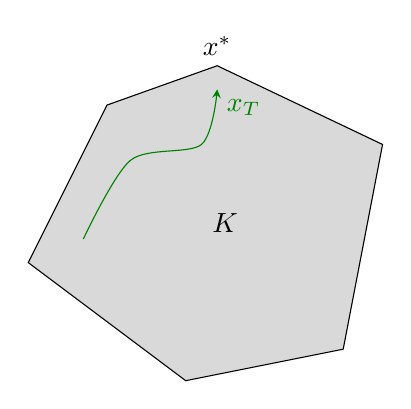
\begin{tikzpicture}[scale=1]
			\draw[fill=gray!30] (0, 0) -- (2, 0.4) -- (2.5, 3) -- (0.4, 4) node[above] {\( x^{*} \) }-- (-1, 3.5) -- (-2, 1.5) -- cycle;
			\draw node at (0.5, 2) {\( K \) };
			\draw [green!50!black, -stealth] plot [smooth] coordinates {(-1.3, 1.8) (-0.7, 2.8) (0.2,3) (0.4, 3.7)}
				node[below right] { \( x_T \) };
		\end{tikzpicture}
	\end{center}

%	\begin{center}
%		\includegraphics[scale=0.9]{ipm.png}
%	\end{center}
	In theory, our point \( x_n \) equals \( x^{*} \) when \( \eta \to \infty \) and \( T \to \infty \). 
	As this is not possible 
	in a finite process, the best we can hope to do is to get approximately close to \( x^{*} \), which echoes 
	what we mentioned earlier about the lack of a finite algorithm for solving SDPs. 

	As this is an iterative method, the runtime of this algorithm is heavily dependent on the number of iterations
	\( T \) we choose to run, and here we come to the main issue for IPM algorithms: each Newton step is an 
	incredibly costly computation, since it requires calculating a matrix inverse and a matrix multiplication. 
	Classically, the fastest known matrix multiplication algorithm runs in \( O(n^{2.37}) \)
	\footnote{This algorithm 
		is also considered a ``galactic algorithm'', or in other words, extremely impractical, and in practice 
		the slower (but much easier) Strassen's algorithm is used instead, which has a runtime of roughly 
	\( O(n^{2.8}) \).}, and the fastest matix inverse algorithms run close to \( O(n^3) \), both of which are 
	incredibly slow \cite{tonksFastMatrixInversion2019}.  

	With this in mind, there are several approaches we can take to easing the computational burden here. Perhaps 
	the most obvious way is to find a faster way to perform matrix multiplication and inversion, which is a valid 
	approach, however it's hard to imagine that this will generate appreciable speedup as it does nothing to affect 
	the number of iterations we have to compute. On the other hand, 
	a more promising approach, and one that we will focus on 
	in subsequent sections, lies in finding ways to shrink the matrices \( H \) and \( g \) to make them more 
	tractable, by way of approximations. This lessens the computational burden in two ways: first, a smaller \( H \)
	and \( g \) maeans calculating \( H^{-1} \) and multiplying it with \( g \) is faster, and second, 
	approximations reduce the number of times we need to compute Newton's step. 


In sum, there are three main steps that incur a high computational cost when using an IPM which are the following:

\begin{enumerate}
\item Calculating and storing the Hessian matrix $H(x)$ and the gradient $g(x)$
    \item Calculating the inverse of the Hessian matrix $H(x)^{-1}$.
    \item Calculating the matrix-vector product $H(x)^{-1}g(x)$.
\end{enumerate}

Putting these elements together, the best classical runtime achieved is somewhere on the order of \( \widetilde
O(nd + d^{3})\). As we'll see, the quantum algorithm we focus on has an optimal runtime of \( \widetilde O(
\sqrt{n} \ \mathrm{poly}(d)\), which is much faster. 

	\section{Quantum IPM Algorithms} 
	Now that we are familiar with the problem and challenges in implementing an efficient algorithm classically, 
	we move to investigating how quantum algorithms can be used to generate speedup for these operations. In 
	particular, we will focus on the paper by Apers and Gribling, who propose a new quantum IPM algorithm that 
	bypasses many of the challenges encountered by the algorithms that precede it. 

	Before we begin discussing the algorithm, it is useful to first take a look at some elements of quantum computing 
	that will be instrumental in showing a speedup over classical algorithms. 

	\subsection{Quantum Random Access Memory}
	One subroutine this paper, along with many other papers employ is the quantum implementation of classical 
	random access memory, also called QRAM. In essence, this subroutine provides an \( O(n) \to O(\log n) \) speedup in 
	query length, and is one of the major subroutines used to achieve a better runtime. 

	The philosophy behind QRAM is relatively simple: instead of accessing a single memory location, 
	QRAM uses superposition to access multiple memory locations at once. This can be implemented in different ways, 
	one of which is the ``bucket-brigade'' implementation, detailed in \cite{giovannettiQuantumRandomAccess2008}. 
	To explain how this works, consider a classical 
	RAM with \( n \) bits, which encodes for \( 2^{n} \) memory locations. Now, since there are \( 2^{n} \) locations, 
	we can imagine each memory location being a leaf in a full binary tree with \( n \) layers:  

	\begin{center}
		\begin{forest}
			[\( \cdot \) [\( 0 \) [\( 0 \) [ \( X_{00} \)]] [\( 1 \) [\( X_{01} \) ]]] [\( 1 \) 
			[ \( 0 \) [\( X_{10} \) ]] [\( 1 \) [ \( X_{11} \) ]]]]
		\end{forest}
	\end{center}
	Then, the data at location \( X_{ab} \) can be specified by the binary string \( ab \), where the value of 
	\( a \) and \( b \) trace the path from the root node to the leaf in question. Note that the path 
	is traced from most to least significant bit -- for instance, \( X_{01} \) 
	is encoded by the bits \( a = 0, b = 1 \). 

	Quantumly, the idea is more or less the same, except now, each node is replaced by a three-state system, 
	sometimes called a qutrit. The states are \( \ket*{\cdot}, \ket*{0} \) and \( \ket*{1} \). The \( \ket*{\cdot} \) 
	state is referred to as a ``wait'' has the special property that whenever a state, either \( \ket*{0} \) 
	or \( \ket*{1} \) is received, the state transforms into the received state. That is, if it receives \( \ket*{0} \),
	then \( \ket*{\cdot} \to \ket*{0} \), and the same goes for \( \ket*{1} \). Then, to access a particular 
	cell, we specify the path to that cell by feeding in the path one qubit at a time, 
	just like we did classically; the diagram below shows an example 
	where we try to access \( \ket*{X_{01}} \):

	\begin{center}
		\begin{forest}
			[\( \cdot \) [\textcolor{red}{\( \ket*{0} \)} [\( \ket*{\cdot} \) [ \( \ket*{X_{00}} \)]] 
			[\textcolor{red}{\( \ket*{1} \)} 
			[\textcolor{red}{\( \ket*{X_{01}} \) }]]] [\( \ket*{\cdot} \) 
			[ \( \ket*{\cdot} \) [\( \ket*{X_{10}} \) ]] [\( \ket*{\cdot} \) [ \( \ket*{X_{11}} \) ]]]]
		\end{forest}
	\end{center}
	the red markers indicates the path taken to \( \ket*{X_{01}} \). Now, how is this faster than the classical 
	approach? Well, the key comes when we consider superpositions of states. What if, instead of feeding in  
	just \( \ket*{0} \) or \( \ket*{1} \), we instead fed \( \ket*{+} = \frac{1}{\sqrt{2} }(\ket*{0} + \ket*{1}) \) 
	twice? Well, then both paths would be activated due to superposition, and as a result instead of getting a single 
	qubit as earlier, we would get a superposition of all four memory states: 
	\[
	\frac{1}{2}(\ket*{X_{00}} + \ket*{X_{01}} + \ket*{X_{10}} + \ket*{X_{11}})
	\] 
	In general, for a QRAM of \( n \) qubits, if we gave \( \ket*{+}^{\otimes n} \) as an input (in succession), 
	then the output 
	would just be a superposition of all the memory states. This is the power of QRAM -- with  
	only \( n \) queries, we managed to access \( 2^{n} \) different memory locations, or equivalently, for \( n \) 
	memory locations we only ened \( \log n \) queries. This is why QRAM introduces an \( O(n) \to 
	O(\log n)\) speedup.   

	As we'll see, QRAM is one of the central subroutines that are assumed to be implemented in the algorithm we 
	will focus on. This is also true for many other quantum algorithms out there -- they assume access to 
	QRAM, and as a result they are able to claim a \( O(n) \to O(\log n) \) query time basically for free.  


\subsection{Quantum Gradient Estimation}

Gradient estimation has been an area of major research for quantum algorithms. 
One of the first such algorithms is Jordan's algorithm \cite{} which supposes black-box access to a function 
and can compute the gradient of said function in constant time. 
This algorithm is of little practical use for this problem, 
however, as we have analytical access to the functions in question. Another approach is a parameter shift technique for 
 
 
\subsection{Main Result}
Previously, one of the main challenges in devising an efficient quantum SDP solver is that regardless of 
the method chosen, there was always dependence on what is called a \textit{condition number}. In essence, 
the dependence on a condition number implies that the runtime of the algorithm was highly dependent on the 
values to the input matrices; this is problematic because it means that the runtime of such algorithms 
varies wildly depending on the values to the input matrix. However, this algorithm we will focus on removes 
that dependence entirely, and as such is seen as a monumental achievement in the search for a faster 
quantum IPM algorithm. 

In particular, this algorithm develops two main subroutines \cite{}:
\begin{enumerate}[label=\alph*)]
	\item An efficient algorithm to spectrally approximate the Hessian. 
	\item An efficient algorithm to approximate a matrix-vector product. 
\end{enumerate}
The implementation of these algorithms allow us to calculate an approximate Hessian \( Q(x) \) and gradient 
\( \tilde g(x) \), which is then used to approximate the update step via \( \tilde n(x) = -Q(x)^{-1} \tilde g(x) \).
To be more specific, the form of \( g(x) \) allows us to write it in terms of a matrix-vector product, which we 
then use the latter subroutine to efficiently approximate it. 

\subsection{Quantum Spectral Approximation}
As this is one of the main subroutines the paper leverages, it is one that is important to look at if one is to 
understand the entire algorithm. As outlined in Theorem 3.1 of \cite{}, 
the following is the formal statement of the spectral 
approximation:

\begin{theorem}[Quantum Spectral Approximation]
	Consider query access to a matrix \( B \in \R^{n \times d} \) with row sparsity \( r \). For any \( 0 < 
	\epsilon \le 1\), there is a quantum algorithm that, with high probability, returns a matrix \( \tilde B^{
	\widetilde O(d / \epsilon^2) \times d} \) satisfying 
	\[
		(1 - \epsilon) \tilde B^{\top} \tilde B \preceq B ^{\top} B \preceq (1 + \epsilon) \tilde B^{\top} \tilde B
	\] 
	while making \( \widetilde O(\sqrt{nd}  / \epsilon) \) row queries to \( B \), and taking time 
	\( \widetilde O(r\sqrt{nd} / \epsilon + d^{\omega}) \).  
\end{theorem}
Intuitively, this theorem is best undestood as the following: given a matrix \( B \) in \( \R^{n \times d} \), 
we can use this algorithm to find a matrix \( \tilde B \) such that \( \tilde B^{\top} \tilde B \) is 
within \( \epsilon \) of the true value of \( B^{\top} B \).\footnote{More accurately, we should say that 
	if \( A \preceq B \) then this is the same as \( 0 \preceq B - A \), or in other words the matrix \( B - A \) is 
positive semidefinite. However, the analogy of ``values'' suffices for a conceptual understanding.}  

The reason this spectral approximation is phrased in this way is in part due to the form of the Hesssian matrix 
for \( f(x) \). In summary, becuase all the Hessian matrices considered in the paper are of the form 
\( B^{\top}B \), then the above algorithm perfectly allows us to approximate \( H \).  

The method in which this is done is actually qutie complicated -- the authors make use of an algorithm called 
the \textit{repeated halving algorithm} developed in \cite{cohenEll_pRowSampling2014}. 
In essence, the algorithm works in two parts: first, 
a set of matrices \( A_1, \dots, A_{L} \) is recursively constructed by subsampling \( A \); in other words, 
to generate \( A_{i + 1} \), we keep each row in \( A_i \) with probability \( \frac{1}{2} \). This is then 
combined another subsampling procedure that allows us to construct a matrix \( B_i \) from each \( A_i \). In 
the paper, this is denoted as the step \( B \overset{w, \epsilon}{\leftarrow} A \). Here, instead of each row 
being kept with uniform probability, there is a distribution \( p_i \) instead, which is dependent on the 
dimension of \( A \) along with other factors. This process is recursively done, and once all the 
computation is done we are left with a matrix \( B \) which approximates \( A \) in the sense 
that \( B^{\top}B \approx A^{\top}A \).
 
Quantumly, this latter process of \( B \overset{w, \epsilon}{\leftarrow} A \) is interesting, because its quantum 
implementation is actually rather simple. In particular, this step is actually implemented via Grover search 
\cite{apersQuantumSpeedupGraph2023}, which 
is used to select the rows in \( A \) that we want to use to construct \( B \). It should also be noted that 
this step in particular is one that benefits greatly from QRAM access, since accessing multiple rows of \( A \), which 
is necessary to construct \( B \) would be made far more efficient with QRAM as we can access all these rows 
at once.  
 
This result is then used in conjunction with calculations of leverage scores and Lewis weights in order to 
fully compute an approximation to \( H(x) \). However, the process by which the Lewis weights 
are calculated are relatively complicated, and we will not analyze them in detail in this report. However, 
we will point to \cite{apersQuantumSpeedupsLinear2024} for further reading.  

\subsection{Quantum Matrix-Vector Approximation} 
Perhaps the more interesting of the two subroutines introduced is this efficient method of calculating 
the matrix-vector product. This is stated as Theorem 5.1 in \cite{apersQuantumSpeedupsLinear2024}:

\begin{theorem}[Approximate matrix-vector product]
	Assume query access to a vector \( v \in \R^{n} \) and a matrix \( B \in \R^{n \times d} \) with 
	row sparsity \( r \). There is a quantum algorithm that returns a vector \( \tilde y \) satisfying 
	\[
		\|\tilde y - B^{\top} v\|_{(B^{\top} B)^{-1}} \le  \delta
	\] 
	while making \( \widetilde O(\sqrt{n} d \|v\|_{\infty} / \delta) \) row queries to \( B \) and \( v \), and 
	taking time \( \widetilde O(r \sqrt{n} d^2 \|v\|_{\infty} + d^{\omega}) \).
\end{theorem}
In other words, this algorithm takes in an input \( B\in \R^{n \times d} \)	and \( v \in \R^{n} \), and 
finds a vector \( \tilde y \) that gets arbitrarily close (becuase we 
choose the value of \( \delta \)) to the value of \( B^{\top} v \), which is the matrix vector product. In the 
context of our IPM algorithm, this is the algorithm that finds an approximation to the quantity equivalent 
to the quantity \( Q(x)^{-1}\tilde g(x) \). 

Similar to the spectral approximation, the implementation of this algorithm is also rather complex, and uses 
other algorithms such as the quantum multivariate mean estimation from 
\cite{cornelissenNearOptimalQuantumAlgorithms2022} to arrive at a result. Despite this, the main points 
are relatively easy to understand. First, the input matrix \( B \) is spectrally approximated as \( \tilde W \) 
using the spectral approximation we talked about earlier as a subroutine. This outputs \( \tilde W \), which we then 
convert to \( \tilde W^{ - 1 / 2} \) classically. Now, this quantity is used in conjunction with \( v \) to 
generate a random variable \( X \) from which the quantum multivaraite mean subroutine is used, ultimately 
returning a vector \( \tilde \mu \). Then, we return \( W^{ 1 / 2} \tilde \mu = \tilde y\) as the approximation. 

While the details as to \textit{why} the algorithm works is rather technical, the important point is the following: 
the quantum multivaraite mean algorithm is incredibly efficient, and the authors get around having to 
explicitly approximation \( B^{\top} v \) by using this algorithm to output an estimate \( \tilde \mu \) which 
we use to output \( \tilde y \). 
 

\subsection{Putting it all Together}
Now, we are ready to put everything together. Recall in section \ref{IPM}, we discussed that depending on the way 
we encode our barrier function \( f(x) \), the resulting time (and space) complexity of the quantum algorithm is 
different. In \ref{apersQuantumSpeedupsLinear2024}, the authors detail the implementation of their quantum 
algorithm for three different barriers, of which we will focus on the fastest one: the lewis weight barrier. 
   
The idea of a Lewis weight barrier is inspired by \cite{leeSolvingLinearPrograms}, which defines \( f(x) \) 
as follows:
\[
f(x) = \ln \det(A^{\top}S_x^{-1} W_x^{1 - \frac{2}{p}}S_x^{-1}A) \quad \text{where}\quad 
W_x = \mathrm{Diag}(w^{(p)}(S_x^{-1}A))
\] 
Where \( A \) is the input matrix, and \( S_x \) is a matrix calculated based on the Lewis weights, which as 
mentioned, is a process that we do not fully understand, and will not discuss in detail here. The reason 
this approach is used is because the gradient and Hessian matrices take on a relatively nice form:
\[
	g(x) = -A^{\top} S_x^{-1} W_x \mathbf{1} \quad H(x) = A^{\top} S_x^{-1}W_x S_x ^{-1} A
\] 
Then, leveraging the forms of these matrices, we can apply the spectral and the matrix-vector 
approximation algorithms here to approximate these quantities. This is also done in a very clever way: for \( H \), 
instead of spectrally approximating \( H \), we spectrally approximate the quantity \(B = W_x^{1 / 2}S_x^{-1} A \)
outputting a matrix \( \tilde B \), with the guarantee that \( \tilde B^{\top} \tilde B \approx H(x) \). A similar 
approach is done to approximate \( g(x) \), where we allow \( B = W_x^{1 / 2}S_x^{-1}A \) and 
\( v = W_x^{1 / 2} \mathbf 1 \), whose product is equal to \( g(x) \). 

This last step highlights the major contribution of this paper: the authors were able to find a way to separate 
\( H(x) \) and \( g(x) \) in an incredibly clever way, such that we can apply these algorithms like the 
spectral and matrix-vector approximation in order to approximate \( H \) and \( g \) with an extremely fast 
runtime. Then, combining all these steps together, we finally arrive at a runtime of 
\[
	\widetilde O(\sqrt{n} \mathrm{poly}(d, \log(n), 1 / \epsilon))  
\] 
which is incredibly fast. If we only focus on \( n \) (and ignore polylog factors), 
then we can bascally say that this algorithm 
runs in \( O(\sqrt{n}) \) time, which is significantly faster than the \( O(nd + d^3) \) classical runtime.

 
   
  
%\bibliography{ref}

\end{document}
